 \documentclass[12pt]{article}
\usepackage[utf8]{inputenc}
 
\usepackage[margin=1in]{geometry} 
\usepackage{amsmath,amsthm,amssymb}
\usepackage{algorithm}
\usepackage[noend]{algpseudocode}
\usepackage{graphicx}
 
\newcommand{\N}{\mathbb{N}}
\newcommand{\Z}{\mathbb{Z}}
 
\newenvironment{theorem}[2][Teorema]{\begin{trivlist}
\item[\hskip \labelsep {\bfseries #1}\hskip \labelsep {\bfseries #2.}]}{\end{trivlist}}

\newenvironment{definition}[2][Definición]{\begin{trivlist}
\item[\hskip \labelsep {\bfseries #1}]}{\end{trivlist}}

\newenvironment{example}[1][Ejemplo]{\begin{trivlist}
\item[\hskip \labelsep {\bfseries #1}]}{\end{trivlist}}
 
\begin{document}
 
%\renewcommand{\qedsymbol}{\filledbox}
 
\title{El criptosistema de Merkle-Hellman}
\author{Anna Pietrzak\\Diego Kiedanski\\Tobias Winkler\\Criptografía y Teoría de Códigos\\Universidad Complutense de Madrid} %if necessary, replace with your course title
 
\maketitle

\section{Introducción}


%\cite{shamir1984}
%\cite{merkle1978}

Cuando enviamos mensajes por cualquier canal de comunicación siempre nos exponemos al riesgo de que sean leídos por terceras personas antes de llegar a su destino. Supongamos que queremos mandar el mensaje
$$M = \text{COMPLUTENSE}$$
a nuestro compañero Bob. Para evitar que Eva, una tercera persona que de alguna manera ha conseguido interceptar $M$ en su camino, sea capaz de entender lo que le queremos decir a Bob, le podemos mandar una versión \emph{cifrada} de $M$, por ejemplo
$$M' = \text{DPNQMVUFOTF}.$$
Sin embargo, si hacemos eso tenemos que asegurarnos de que el destinatario Bob es capaz de \emph{descifrarlas} y sería ideal si él fuese la única persona con esa capacidad.

Para ese fin ciframos $M$ de tal manera que el resultado $M'$ dependa de una clave $K$. Más formal, podemos pensar en el cifrado como una función
$$e_K : \mathbb{M} \rightarrow \mathbb{M}'$$
que depende de $K$. Aquí $\mathbb{M}$ y $\mathbb{M}'$ serían los espacios de todos los mensajes y mensajes cifrados posibles, respectivamente. En el ejemplo anterior $e_K$ es la función definida por
$$e_K(m_1\ ...\ m_n) = m_1 + K\ ...\ m_n+K$$
donde la adición de una letra $m$ más un número entero $K$ significa avanzar $m$ por $K$ posiciones en el alfabeto (posiblemente volviendo de Z a A) y la clave que elegimos fue $K = 1$.

Solo las personas que disponen de $K$ serán capaces de entender, es decir descifrar, el mensaje original $M$. Igual que antes, podemos considerar este proceso como otra función
$$d_K : \mathbb{M}' \rightarrow \mathbb{M}$$
nuevamente dependiente de $K$. Entonces, en el ejemplo $d_K$ sería dado por
$$e_K(m_1\ ...\ m_n) = m_1 - K\ ...\ m_n - K.$$
¡Ahora solo nos tenemos que preocupar de que Bob sepa $K$ y ya estaremos listos para mandarle todos los mensajes que queramos!

\subsection*{Cifrado asimétrico}

¿Pero cómo nos podemos comunicar con Bob para intercambiar $K$? En realidad, eso es equivalente a enviar un mensaje con el contenido $K$ y si ese mensaje es interceptado, entonces la comunicación ya no es segura.

Para evitar este problema se han inventado los \emph{cifrados asimétricos}. Usan por lo menos dos claves, una clave \emph{secreta} $S$ y una clave \emph{pública} $P$. Para que le podamos enviar un mensaje a Bob necesitamos saber su clave pública $P$ y él va a tener que usar su clave privada $S$ para descifrarla. Con la notación de antes, el cifrado es una función $e_P$ dependiente de $P$ y el descifrado es $d_S$ que depende de $S$. El cifrado debe ser tal que sea muy difícil (en la práctica imposible) invertir $e_P$ solo conociendo la clave pública $P$.

\section{El cifrado de Merkle-Hellman}

Este criptosisteme es un ejemplo de cifrados asimétricos. Fue inventado por Merkle y Hellman en 1976 \cite{merkle1978}. Fue roto en 1984 por A. Shamir que presentó un algoritmo eficiente (polinomial) que es capaz de recuperar el texto cifrado solo a partir de la clave pública con alta probabilidad \cite{shamir1984}. Por lo tanto, este sistema \emph{ya no se debe usar en la práctica}. (??Más abajo veremos como se puede mejorar el sistema para recuperar la seguridad??) Antes de explicar como funciona tenemos que introducir un poco de teoría.

\subsection*{El problema de la mochila}

Una variante del \emph{problema de la mochila} es la siguiente cuestión: Dado una secuencia $M = m_1, ..., m_n$ de números enteros positivos (la \emph{mochila}) y un \emph{límite} $L$, ¿existen indices $I \subseteq \{1,...,n\}$ tal que $\sum_{i \in I}m_i = L$? Y si existen, ¿cuáles son? Esto también se conoce como el \emph{problema de la suma de subconjuntos}.

\begin{example}
Considera $M = 13, 1, 6, 3, 10$. Si $L = 20$, entonces el problema de la mochila relacionado tiene solución ya que $1+6+3+10 = 20$. Por otra parte, si $L = 8$ no tiene solución porque ninguna combinación de estos cinco números da $8$ en su suma.
\end{example}
%, el \emph{problema de la mochila} consiste en encontrar un subconjunto $S \subseteq M$ que maximice $R := \sum_{s \in S}s$ bajo la restricción que $R \leq L$.
%Un problema relacionado es el \emph{problema de la suma de subconjuntos}. Aquí la pregunta es: ¿Existe $S \subseteq M$ tal que $\sum_{s \in S}s = L$? Ese problema se puede considerar como un caso especial de él de la mochila y sigue siendo NP-completo. A continuación vamos a referirnos a este problema cuando decimos 'el problema de la mochila'.
Se ha demostrado que el problema de la mochila es NP-completo. El algoritmo más simple para resolverlo prueba todas las $2^n$ posible combinaciones de elementos de $M$. Para cada combinación el algoritmo tiene que sumar como máximo $n$ números. Sumar dos números de $r$ bit son se hace en $O(r)$ operaciones, y por lo tanto este algoritmo trivial está en $O(nr2^n)$ si los tamaños en bit de los números en $M$ están limitados por $r$. Como este algoritmo es exponencial en $n$, no se puede aplicar si $n$ es suficientemente grande. Existen mejores algoritmos que este pero el hecho de que el problema es NP-completo nos asegura que ninguno de ellos es polinomial (lo que no significa que no puede haber algoritmos que sean eficientes en muchos casos).

Como vamos a ver, la seguridad del cifrado se va a basar en la dificultad de resolver el problema de la mochila.

\subsection*{Mochilas supercrecientes}

En casos especiales, el problema de la mochila es fácil de resolver como vamos a ver enseguida.

\begin{definition}{1}
Sea $M = m_1, ..., m_n$ una secuencia ascendiente de números enteros positivos. Si $M$ verifica que
$$m_{i+1} \geq \sum_{k=1}^im_k$$
entonces $M$ se llama \emph{mochila supercreciente (MS)}.
\end{definition}
\textbf{Ejemplo}
\begin{itemize}
\item
$M := 3, 4, 11, 42$ es una MS porque $4 > 3$, $11 > 3 + 4 = 7$ y $42 > 3 + 4 + 11 = 18$.

\item 
Para $n \in \N$, $M := 2^0, 2^1, ..., 2^n$ también es una mochila supercreciente ya que todo $i \in \N$ verifica que
$$2^{i+1} - 1 = \sum_{k=0}^i2^k.$$
\end{itemize}
La secuencia del último ejemplo es la 'menor' MS posible, es decir todos los elementos $m_i$ de cualquier MS verifican que $m_i \geq 2^{i-1}$. Esto implica que los elementos de todas las MS de longitud $n$ se representan con por lo menos $n-1$ bits y su suma tiene al menos $n$ bits.

Observamos que si $M = m_1, ..., m_n$ es supercreciente y $m_n \leq L$, entonces si $M$ tiene una solución, es necesario que $m_n$ esté en la solución porque si no, no podremos alcanzar $L$ ya que $m_n$ es mayor que la suma de todos los demás elementos de $M$.
De esta observación podemos concluir el siguiente algoritmo:
\vspace{1em}
\begin{algorithmic}[1]
\Procedure{ResolverMS}{$m_1,...,m_n$, $L$}
\State $sol \gets \emptyset$
\For{$i = n,...,1$}
	\If{$m_i \leq L$}
		\State $sol \gets sol \cup \{m_i\}$
		\State $L \gets L - m_i$
	\EndIf
\EndFor
\State \textbf{return} $sol$
\EndProcedure
\end{algorithmic}
\vspace{1em}
El algoritmo asuma que $M = m_1,...,m_n$ es una mochila supercreciente y que los $m_i$ están en orden ascendiente. Su complejidad de tiempo es $O(n)$ (lineal en $n$) porque consiste de un solo bucle de exactamente $n$ iteraciones.

\subsection*{Cifrar y la clave pública}

Para cifrar un bloque $B = b_1...b_n$ de $n$ bits tomamos una mochila supercreciente $M = m_1, ..., m_n$ de longitud $n$. Entonces eligimos dos números $q, r \in \Z$ tal que $q > \sum_{i=1}^nm_i$, $r > 1$ y el máximo común divisor de $q$ y $r$ sea $1$. Llamamos \emph{modulo} a $q$ y \emph{multiplicador} a $r$. Se sugerieron valores alrededor de $n = 100$ y $q$ de $200$ bits. Calculamos
$$M' = \{m_1', ..., m_n'\} = \{r m_1 \text{ mod } q, ..., r m_n \mod q\}.$$
Es importante entender que $M'$ en general ya no es supercreciente debido a las operaciones de modulo. Obtenemos el bloque cifrado $B'$ sumando aquellos elementos de $M'$ cuyos indices corresponden a los bits que valen uno en nuestro bloque $B$, es decir hacemos la suma
$$B' = \sum_{i=1}^nb_im_i'.$$
$B'$ es un solo número en $\Z$.

¿Cómo obtenemos una mochila supercreciente? Se puede generar una MS aleatoriamente de la siguiente manera: Se elige un parametro $\texttt{salto}\ > 1$. Sean $a_1, ..., a_n$ elementos tomados de la distribución uniforme de los números enteros de $1$ a \texttt{salto}. Definimos $m_1 := a_1$ y $m_{i+1} := a_{i+1} + \sum_k^n m_{k}$. Entonces $m_i \leq \texttt{salto} \cdot 2^{i-1}$ por inducción:
\begin{itemize}
	\item $i = 1$: $m_1 \leq \texttt{salto}$ es correcto
	\item $i > 1$:
	$$m_{i} = a_i + \sum_{k=1}^{i-1} m_{k} \leq a_i + \texttt{salto} \cdot \sum_{k=1}^{i-1}2^{k-1} \leq \texttt{salto} + \texttt{salto} \cdot ( 2^{i-1} - 1) = \texttt{salto} \cdot 2^{i-1}$$
\end{itemize}
Entonces, el tamaño en bit de los $m_i$ no es más de $log_2(\texttt{salto}) + (i-1)$. Lo ideal sería tener un método que genere uniformemente una MS del conjunto de todas las MS con elementos acotados por un límite que queramos. Con nuestro método podemos obtener mochilas con todos los $m_i \leq \texttt{salto} \cdot 2^{n-1}$ como hemos visto, pero no generamos \emph{todas} las posibilidades: Por ejemplo, si $\texttt{salto} = 2$ y $n = 5$, el método garantiza que $m_i \leq 2 \cdot 2^{5-1} = 32$, pero la MS
$$1,2,4,8,32$$
es imposible obtener ya que el salto entre $8$ y $32$ es mucho más grande que el mayor salto posible, que es $2$. En realidad el método solo genera un subconjunto relativamente pequeño de todas las posibilidades. Aquí le daríamos a un atacador la posibilidad de pensar como puede aprovechar esta estructura muy específica de nuestras MS. Sin embargo, para la implementación del sistema que solo sirve como demostración del mismo, este método parecía suficiente y adecuado ya que era muy fácil de implementar.

\begin{example}
Supongamos que queremos cifrar el número 157. Su representación binaria es $B = 10011101$. Entonces, como explicado antes, tenemos que eligir una mochila supercreciente de longitud $8$, por ejemplo
$$M = \{1, 3, 6, 11, 27, 53, 111, 213\}$$
y los números $r$ y $q$. Como la suma de todos los elementos en $M$ es igual a $425$, podemos tomar $q = 499$ y $r = 101$. Como $101$ es primo, $mcd(q,r) = 1$. La mochila $M'$ resultante sería
$$M' = \{101, 303, 107, 113, 232, 363, 233, 56\}$$
que claramente no es supercreciente. Ya podemos calcular el bloque cifrado:
$$B' = 101 + 113 + 232 + 363 + 56 = 865$$
\end{example}
Para cifrar solo se necesita la mochila transformada $M'$, por eso la clave pública es $K_P = M'$.

\subsection*{Descifrar y la clave secreta}
Como da igual si primero sumamos y después tomamos modulo o al revés, la siguiente equivalencia es correcta:
$$B' = \sum_{i=1}^nb_i(rm_i \mod q) \equiv r\big(\sum_{i=1}^nb_im_i\big)\mod q$$
y por lo tanto
$$\sum_{i=1}^nb_im_i \equiv r^{-1} \cdot B' \mod q.$$
$r^{-1}$ existe porque $mcd(r,q) = 1$. Ahora para averiguar los $b_i$ solo tenemos que resolver el problema de mochila con $M$ supercreciente y eso se puede hacer muy rápido como hemos visto antes.

\begin{example}
Tenemos $r^{-1} = 101^{-1}= 84 \mod q$ lo que se puede calcular eficientemente con el algoritmo extendido de Euclides. Entonces,
$$r^{-1} \cdot B' = 84 \cdot 865 \equiv 305 \mod 499.$$
Lo único que falta es llamar el algoritmo \textsc{ResolverMS}($M, 305$) que nos da el resultado $305 = 1 + 11 + 27 + 53 + 213$. Estos números de la mochila $M$ corresponden precisamente al bloque original $10011101$.
\end{example}
Para descifrar se necesita $r^{-1}, q$ y la mochila original $M$, por lo tanto tenemos la clave secreta $K_S = (M, r^{-1}, q)$.

\section{Implementación}

Hemos implementado el sistema de Merkle-Hellman en Python. Existen los scripts \textbf{key\_generator}, \textbf{encrypt} y \textbf{decrypt} que se utilizan como se explica a continuación:

\begin{itemize}
	\item \textbf{python key\_generator.py \textit{n} \textit{jump}}: Crea dos archivos \textit{clave.priv} y \textit{clave.pub} que forman una pareja de claves. Se van a generar claves (mochilas) de longitud $n$ y saltos entre $n$ y \textit{jump} como se ha explicado anteriormente.
	\item \textbf{python encrypt.py \textit{key} \textit{message}}: Genera el archivo \textit{message.crp} que se obtiene cifrando \textit{message} con la clave pública \textit{key}.
	\item \textbf{python decrypt.py \textit{key} \textit{message}}: Genera el archivo \textit{message.dcrp} que es el resultado de descifrar el mensaje \textit{message} con la clave secreta \textit{key}.
\end{itemize}
Aparte de esto también creamos el script \textbf{bruteforce} que, dado un mensaje cifrado y la clave pública, intenta reconstruir el mensaje original resolviendo el problema de la mochila \emph{no supercreciente} tras probar todas las posibles combinaciones. Este programa solo sirve para evaluar la seguridad y no forma parte del criptosistema.

\section{Ataque al criptosistema}

El criptosistema de Merkle-Hellman se considera roto pues existe un ataque en tiempo polinomial al mismo. Lo que es más, el ataque está dirigido a la clave pública, por lo que puede realizarse antes de que las claves sean siquiera utilizadas. La explicación está basada en \cite{stamplattice}.

\subsection{Teoría detras del Ataque}

Sea $T = (t_1,t_2,\dots,t_n)$ la clave pública (mochila) y $M = b_0b_1\dots b_n$ un mensaje (númerico) en base 2 a encripar. El mensaje encriptado es $C = b_0t_1 + b_1t_1 + \dots b_nt_n$ y en forma matricial: $TM = C$. Desencriptar el mensaje es equivalente a encontrar un vector $U = (u_1,u_2,\dots, u_n)$ tal que sea solución del sistema $TU = C$.

No es difícil observar que si definimos $V = (U,1)$ y $W = (U,0)$ entonces vale la siguiente ecuación matricial: $MV = W$, donde 
$$M = \left(\begin{array}{c c}
I_{nxn} & 0_{nx1} \\ T & -C
\end{array}\right)$$

Las columnas de $M$ tienen coordenadas enteras y son linealmente independientes (las primeras n coordenadas forman una base más el vector nulo), por lo que $W$ es un elemento del retículo que forman las columnas de $M$. 

Dado que las coordenadas de $W$ son binarias, $||W|| \leq \sqrt{n}$. Está norma es particularmente pequeña en un retículo de coordenadas enteras. 

El algoritmo de Lenstra–Lenstra–Lovász (LatticeReduction en WolframAlpha \cite{weisstein2010lattice}) permite encontrar vectores de norma pequeña en un retículo con coordenadas en $\mathbb{Z}$. La complejidad de dicho algoritmo es $O(d^5 n log^3 B)$ donde $B$ es el máximo de las normas euclídeas de la base.

El algoritmo toma como entrada la matriz $M$ y devuelve una lista de vectores. Una solución aceptable a nuestro problema no siempre es encontrada pues es posible que las entradas de los vectores no pertenezcan a ${0,1}$.

A pesar de esto, la posibilidad de poder romper una gran cantidad de claves hace que el algoritmo no sea seguro.

\subsection{Ejemplo}

Dada la clave pública $T = [576, 2448, 2767, 237, 330, 2100]$ y el mensaje \textbf{Hola}, se representación en utf8 de 16 bits es: \begin{equation}
\begin{split}
A = 000000\\
000100\\
100000\\
000000\\
011011\\
110000\\
000001\\
101100\\
000000\\
000110\\
000100\\
000000\\
000010\\
100000\\
000000\\
100000
\end{split}\end{equation} y encriptado consiste de la lista de bloques $$C = (0, 237, 576, 0, 7645, 3024, 2100, 3580, 0, 567, 237, 0, 330, 576, 0, 576)$$

Veamos como a partir de la lista $C$ podemos recuperar el mensaje $A$. Lo ejemplificaremos con el quinto elemento de $C: 7645$. Construimos la matriz \begin{equation} M_{7645} = \left( \begin{array}{ccccccc}
1 & 0 & 0 & 0 & 0 & 0 & 0 \\ 
0 & 1 & 0 & 0 & 0 & 0 & 0 \\
0 & 0 & 1 & 0 & 0 & 0 & 0 \\
0 & 0 & 0 & 1 & 0 & 0 & 0 \\
0 & 0 & 0 & 0 & 1 & 0 & 0 \\
0 & 0 & 0 & 0 & 0 & 1 & 0 \\
576 & 2448 & 2767 & 237 & 330 & 2100 & -7645 
\end{array} \right) 
\end{equation}

y utilizamos el algoritmo LLL implementado en Mathematica para obtener la salida (por la implementación de Mathematica debemos suministrar la matriz transpuesta).

En la Figura \ref{wolfram} se puede ver la entrada y la salida del algoritmo. El primer resultado es el que estamos buscando y vemos que coindice con el quinto bloque de $A$ (recordar que hay un 0 al final de sobra).

\begin{figure}
	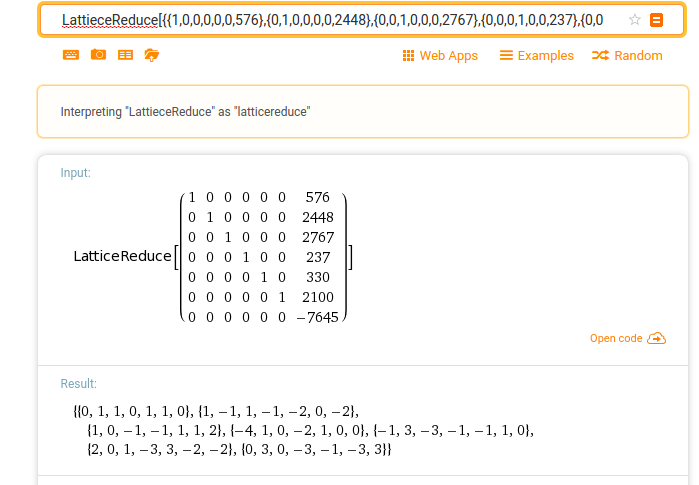
\includegraphics[scale=0.7]{salida_lll}
	\caption{Resultado de la ejecución del algoritmo LLL en Mathematica a la matriz $M_{7645}$}
	\label{wolfram}
\end{figure}

\bibliographystyle{alpha}
\bibliography{references}

 
\end{document}